\mysubsection{Johannes Winter}{Design}

Bedingt durch die Beschränkung durch die Projektionsfläche des Beamers und der menschlichen Körpermaße wurde die Matrix auf 5x8 Felder beschränkt. Die schmale Seite beschreibt die Tonhöhe – jede Reihe ein Ton der Pentatonik. Die breite Seite sind die Tondauern – ein jedes Feld eine Achtel (oder je nach Song im Challenge Mode andere Notenwerte). Die genaue Funktionsweise ist im Abschnitt \ref{sec:music} beschrieben.

Das ursprüngliche Farbschema sah vor, dass entsprechend der Abstufung der Töne auch die Felder in Grautönen abgestuft werden sollten. Von hohen nach tiefen Tönen sollten auch die Felder von Weiß nach Grau eingefärbt werden. Aktivierte Einzelfelder blau, mehrere zusammenhängend aktivierte Felder zur Erzeugung der Mischtöne grün. Der Impuls wurde zunächst violett angedacht und die abgetasteten Felder rot (vgl. Abb. \ref{fig:design}). Da der Boden zu dunkel ist, um die Mischtöne kontrastreich darzustellen, wurde auf diese verzichtet. Statt der Grauabstufungen sind alle Felder weiß. Aktivierte Felder bleiben blau, gerade abgetastete werden grün und erhalten spezielle Effekte, um deutlicher hervorzuheben, dass genau diese Felder gerade vom Impuls abgetastet wurden. Sie shaken und versprühen Partikel. Der Impuls selbst wurde gelb angezeigt.

\begin{figure}[htbp]
\subfigure[Freestyle Modus]{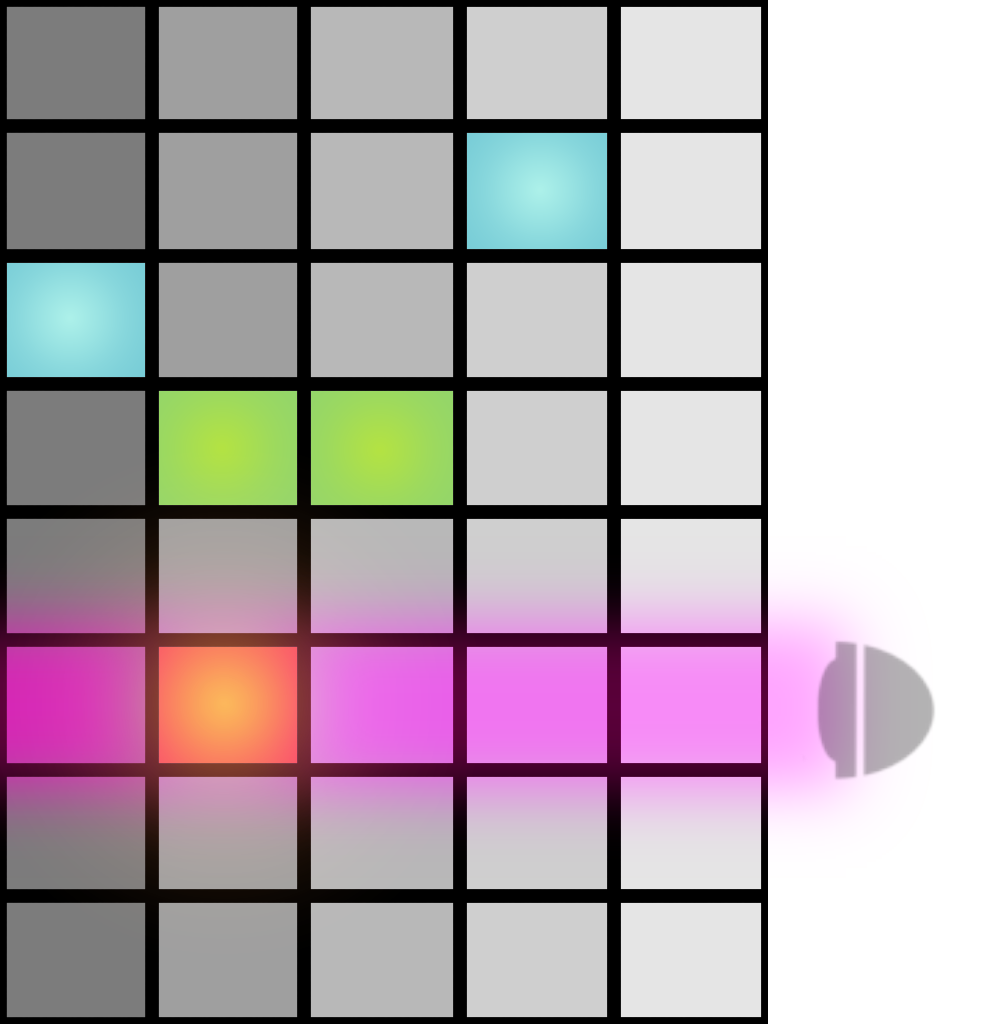
\includegraphics[width=0.49\textwidth]{images/designfelder.png}}\hfill
\subfigure[Idle Modus]{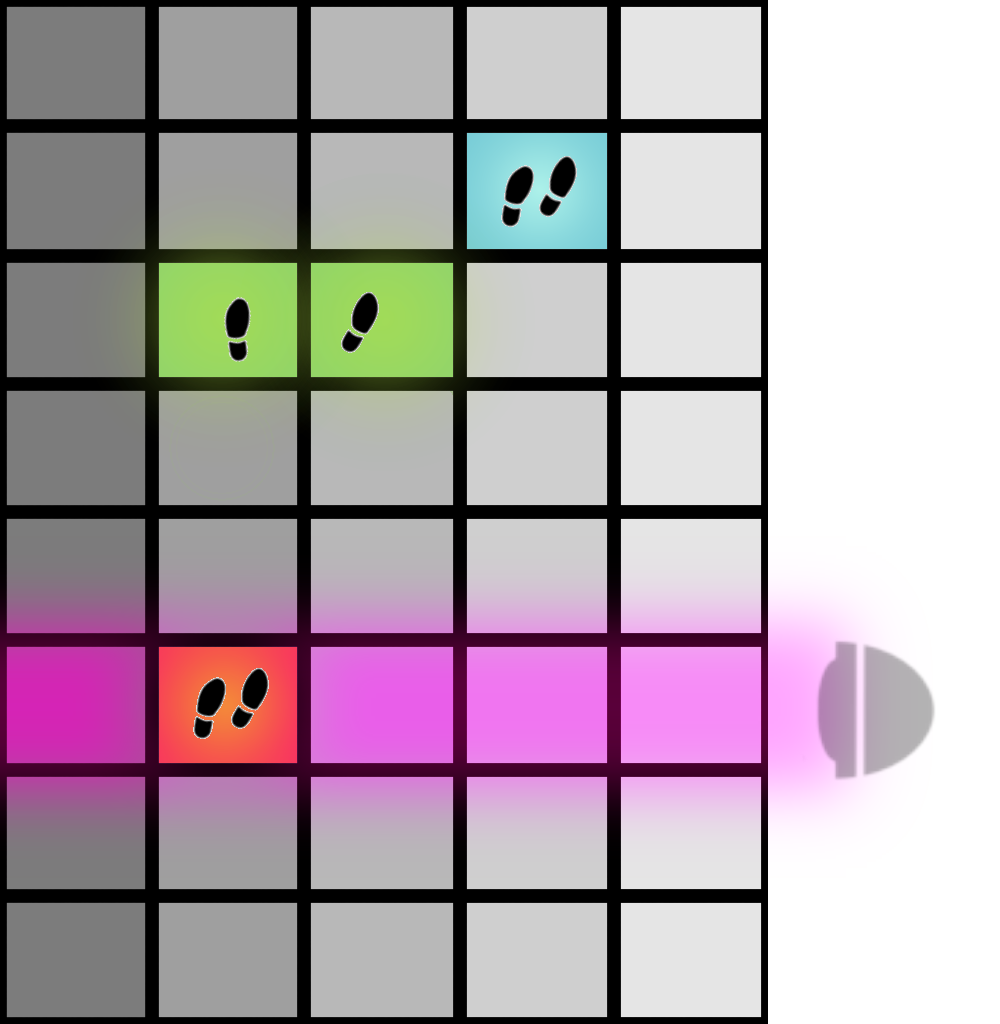
\includegraphics[width=0.49\textwidth]{images/designIdle.png}}
\caption{Ursprüngliches Farbschemas aus der Konzeptphase}
\label{fig:design}
\end{figure}

Im Challenge Mode werden die vorgegebenen Felder blassrot mit blauroter Umrandung angezeigt. Aktivierte Felder sind blau. Ob man richtig steht oder nicht, zeigt sich erst, sobald der Impuls durchläuft. Richtig aktivierte Felder werden grün, falsche rot angezeigt. Im Idle Mode werden in den aktivierten Feldern zusätzlich verschiedene Fußspuren angezeigt. Schuhe, Hunde und Dinosaurier, um das Bild aufzulockern und den spielerischen Charakter von BlinkenTiles zu verdeutlichen.






